\chapter{Software Design and Implementation}

After conducting the required theoretical research, this project sought to implement a Java API for ordering a range different kinds of data, based upon the users topic preferences and the time-of-day, for relevance. This section details the technical design specification of the Java library and the important implementation considerations.

\section{Data Sources and Acquisition}

A host of different kinds of data which are available to smart-phones, are to be used in this project. Their respective sources are available through social media and Google accounts. 

\subsection{Acquisition}

The API does not include the configuration of the data sources, since these are implemented externally to the API for maximum flexibility as to the sources of data used. For example, Facebook statuses \cite{Facebook4JExample} and Tweets \cite{Twitter4JExample} are acquired from their respective APIs, as discussed in the Literature review; the calendar is retrieved by querying Google's Android \emph{ContentResolver}; tasks are queried from the standard Android tasks service and SMS messages through using an intent which returns a Bundle of messages (Appendix \ref{exampleCode}). 

\subsection{DataItem Conversion and Structure}

A \emph{DataItem} is a generalised representation of an item of data of any type. When the item is initially acquired on the device, the software using the API would instantiate a new \emph{DataItem} and set its instance variables (Figure \ref{classes}) with the data from the source object (i.e. a Facebook Status from the Facebook4J API). 

\subsection{UserContext Acquisition and Structure}

The \emph{UserContext} is an object which represents the users topic preferences (Figure \ref{classes}). There are 12 topics which are each given a score between 1 and 10, where 10 indicates a high-priority topic preference. The \emph{UserContext} should be instantiated outside of the \emph{RankingAgent} by using its getters and setters and passed into its constructor. This gives the user of the API maximum flexibility in where to set up the \emph{UserContext}. 

\section{Structure of Implementation}

The API is encapsulated in the \emph{RankingAgent} class (classes referred to are outlined in Figure \ref{classes}). This class abstracts away the complexity of the main stages of the recommender algorithm. The \emph{RankingAgent} contains a \emph{List} of \emph{unsortedDataItems} and the \emph{UserContext}. The \emph{unsortedDataItems} are passed into the \emph{DataContextBuilder} which consructs a \emph{DataContext} object which describes the relevant aspects of the item of data. The \emph{RankingAgent} then passes the \emph{unsortedDataItems} and the \emph{UserContext} into the \emph{Scorer} which is a class for assigning a score to a DataItem. A \emph{List} of scored \emph{DataItem's} is returned to the \emph{RankingAgent} where they are ordered from least to greatest score. 

\begin{figure}[ht!]
	\centering
	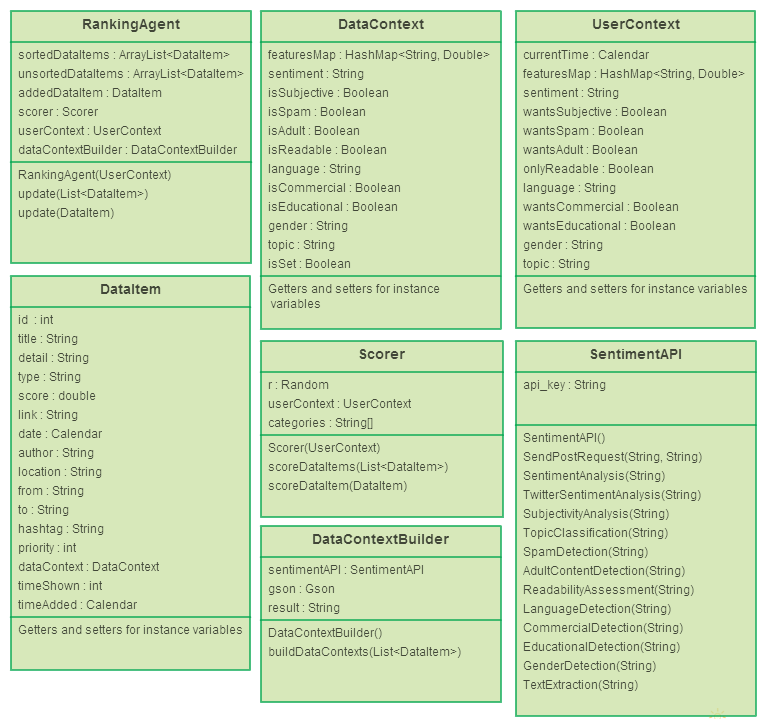
\includegraphics[width=155mm]{images/ProjectClasses.png}
	\caption{Class outlines showing instance variables and public methods}
	\label{classes}
\end{figure}

\subsection{Text Analysis}

The DatumBox \cite{DatumBox} remote textual analytics API is used to collect analytical information about the item of data. Most importantly it assigns the item with a topic and a score of how closely it matches that topic. The SentimentAPI class (outline in Figure \ref{classes}) was implemented to handle the connection of the API to the DatumBox server and detect specific features pertaining to the nature of the content of each item of data. These include the topic classification, spam detection and language detection features among others, which are used in the scoring algorithm. 
The SentimentAPI is used by the \emph{DataContextBuilder} in its construction of the \emph{DataContext} for a \emph{DataItem}. 

\subsection{Scoring Algorithm}

Once the \emph{DataItem} has a \emph{DataItemContext}, it is scored by implementing the proposed novel algorithm (Eqn. \ref{BasicScoringRule3}). \emph{DataItem} objects may be scored as a \emph{List} of \emph{DataItems}, or as single \emph{DataItems}. 
Inside the \emph{Scorer}, the \emph{UserContext} is compared to the \emph{DataContext}. Within each there is a \emph{HashMap} matching a topic (String, Key) to a score (Double, Value) called the \emph{featuresMap}. This is a map of the score of each \emph{feature} or \emph{topic} which may describe the \emph{DataItem}.
If the \emph{DataItem} is of a type such that the criterion that it should be scored by is its time-relevance (i.e. appointment or task), a score is applied based upon whether or not it has reached the time threshold of relevance. If the \emph{DataItem} is of a type such that it should scored based upon its content, the \emph{featuresMap} of the \emph{UserContext} is compared for similarity to the \emph{featuresMap} of the \emph{DataContext} of the \emph{DataItem}.
Since the DatumBox API is limited to quantifying the relevance of only the most appropriate topic for the \emph{DataItem}, the implementation of the recommender algorithm simply compares the relevance of that topic to the corresponding score of the \emph{UserContext} for that topic. 
This \emph{Scorer} class returns a \emph{List} of scored \emph{DataItems}. The \emph{DataItems} are then sorted and returned to the parent class.

\section{Design Considerations}

In the software implementation of the API, there were a number of design decisions which were made in order to maximise the functionality, efficiency and flexibility of the use of the API. 

\subsection{Speed Considerations}

Since the API uses a remote server to perform text analysis on the \emph{DataItem's}, there is incurred a significant delay while waiting for the response to be returned. The DatumBox API is limited in accepting only one string of text per request and as such, text analysis cannot be done in a single POST request to the server. This could not be avoided without using a different text analysis service, however since this is an API for simply demonstrating the behaviour of the recommender system and not a commercially viable prototype, speed is not a huge concern. 
A single request takes approximately 1400 milliseconds, so in order to rank 10 \emph{DataItem's} it takes around 15 seconds. When the other analysis features of the DatumBox API are used this is increased to around 98 seconds to account for the additional requests. 
Computational delay was not considered as there is an insignificant amount of computational processing required for post-analysis scoring. 

\subsection{Usability Considerations}

The recommender system API has a single and simple function and consequently has been designed to have simple usage. 

\lstset{language=Java, caption=API usage example, label=APIUsageExample}
\begin{lstlisting}
// Declare Ranking agent and the List of DataItems to store output
public static RankingAgent rankingAgent;
public static List<DataItem> rankedDataItems = new ArrayList<DataItem>();

// Setup UserContext object from any source
UserContext userContext = getUserContext();

// Load source data from any source
List<DataItem> dataItems = TestDataManager.loadData();

// Instantiate RankingAgent with UserContext
rankingAgent = new RankingAgent(userContext); 

// Call 'update' method to add, analyse, score and sort dataItems
rankedDataItems = rankingAgent.update(dataItems);
\end{lstlisting}

In the command-line application the \emph{Prioritiser} class uses the RankingAgent API to demonstrate its usage (See Listing \ref{APIUsageExample}. A RankingAgent object is instantiated, as is a \emph{List} of \emph{DataItem's} to be used to store the ranked \emph{DataItem's}. A \emph{UserContext} is instantiated and initialised from a stored JSON (JavaScript Object Notation) file, however this can be initialised explicitly. It is passed into the constructor of the \emph{RankingAgent}. The raw items of data are loaded from the JSON-file database in this example and passed into the update method of the \emph{RankingAgent}. This method returns an analysed, scored and ordered \emph{List} of the most relevant \emph{DataItem} objects to the user. 


